\documentclass[../main.tex]{subfiles}
%!TEX root = ./analysisThrusterShaft.tex
\graphicspath {{../}}

\begin{document}
\subsection{Thruster Shaft} \label{thrustShaft}

\begin{figure}[H]
	\centering
	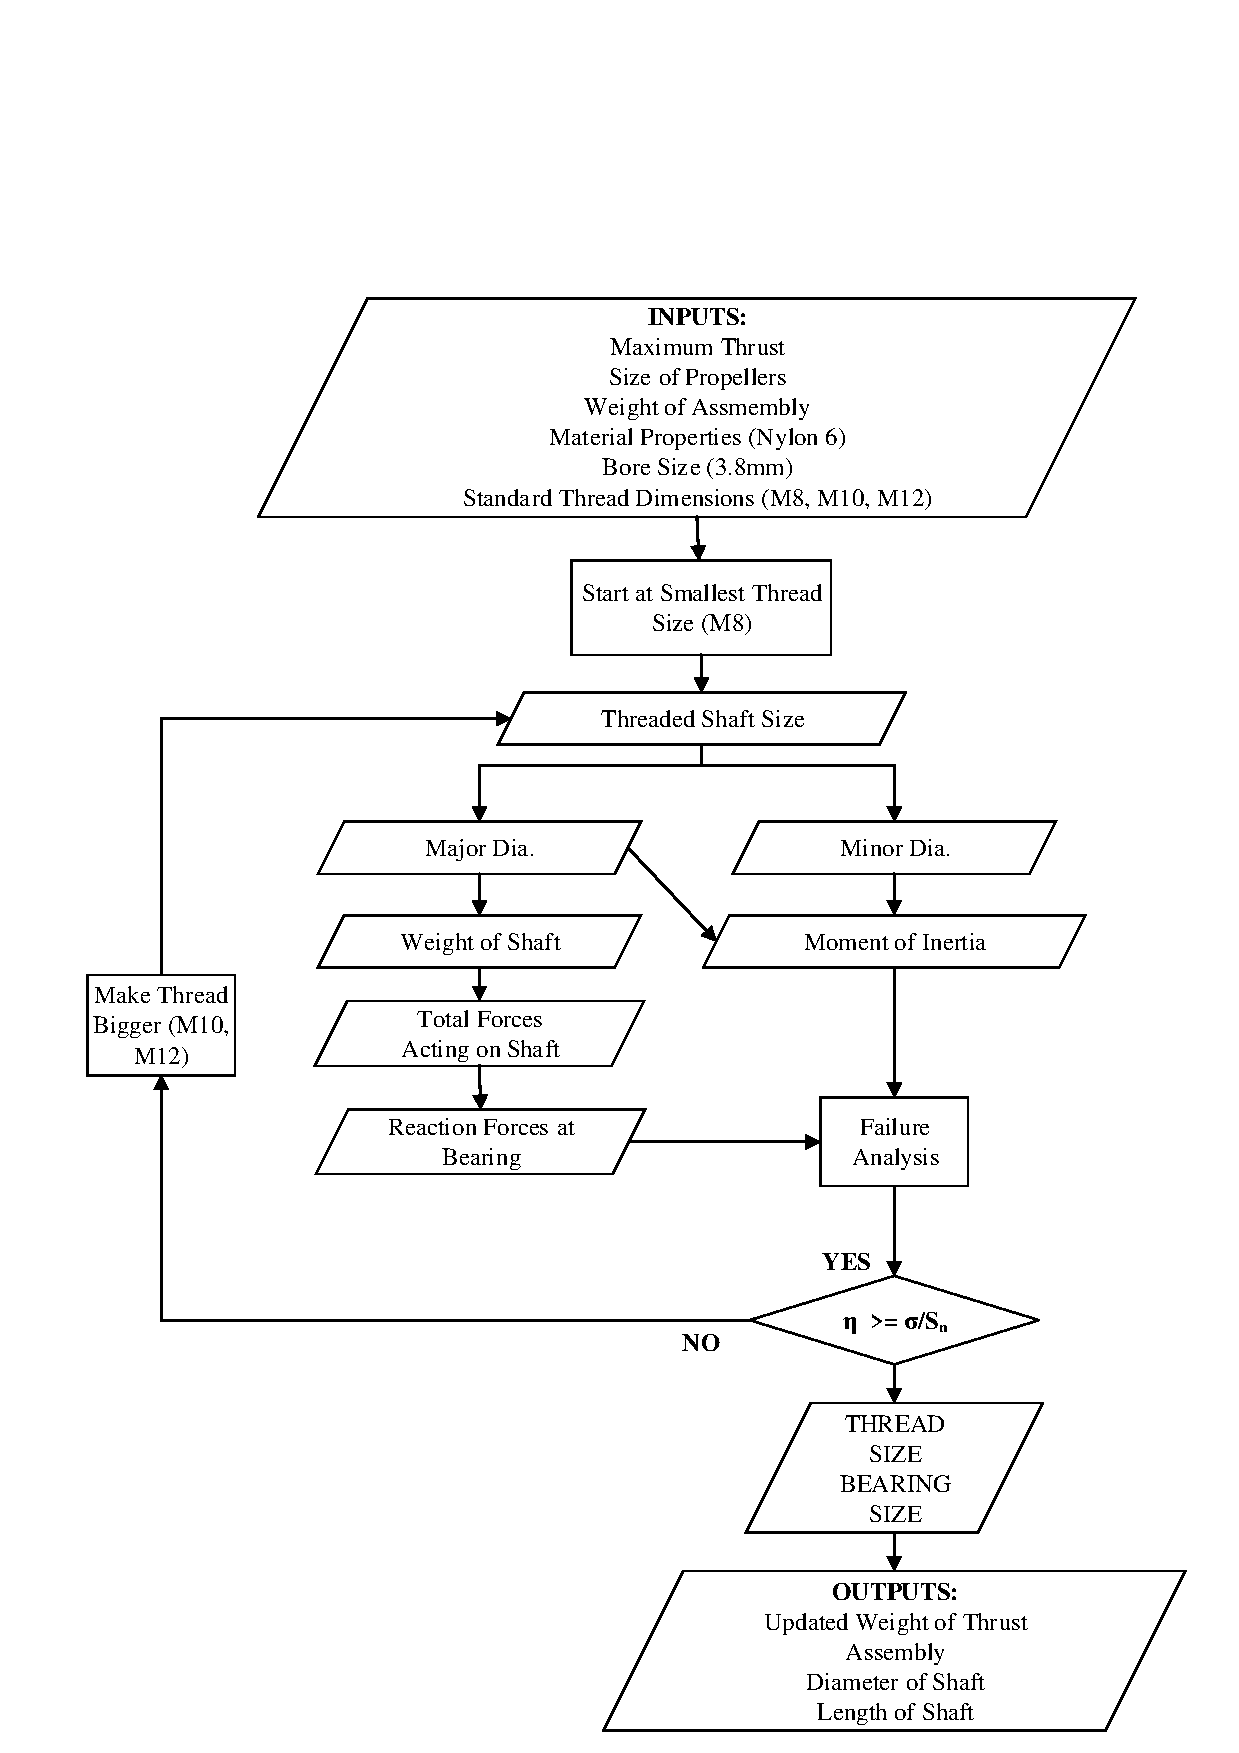
\includegraphics[width=.9\linewidth]{img/paramaterization/thrusterShaft.pdf}
	\caption{Parametrization Outline for the Thruster Shaft}
	\label{fig:ThrusterShaftParametrization}
\end{figure}

The thruster shaft analysis will optimize the diameter of the thruster shaft based on standard threaded shaft dimensions The Analysis will output the diameter of the shaft, the thread of the shaft, the length of the shaft, the weight of the shaft from which it updates the weight and centre of gravity of the entire thruster assembly. The inputs required for the analysis are the maximum thrust, the size of propellers, the weight of the assembly, the material properties of Nylon 6 \cite{Nylon6} (the shaft material), the bore size of the shaft which is 3.8mm and the standard thread dimensions from M8 to M16 REF \cite{threadSizes}.\\

The material nylon 6 was chosen because of its suitable strength, ease of manufacturability and weight. Aluminium was also considered but would have resulted in an over-engineered component or a un-proportionally small radius while still being heavier. Results that justify this decision are shown at the end of the section REF??. The bore diameter of 3.8mm is based on the screw that attaches the shaft axially to the thrust vectoring motor, shown in FIG ??.\\

The scenario for the analysis is that described in Loading Scenario, Section \ref{loadingScenarios}, Maximum Downward Force is shown in Figure \ref{fig:thrusterShaftFBD} where all forces are with reference to the coordinate system $xyz$ defined by the pitch of the airship. The shaft is analysed using simple bending where it is cantilevered at the bearing in the thrust vector motor assembly shown in Figure \ref{fig:thrusterShaftFBD}. The analysis begins by calculating the required length of shaft for the propeller size, as well as the position of the propeller with reference to the bearing. The forces and weigths are passed to forceSolver REF??? to solve the force and moments at the bearing of all the forces acting on the shaft.

\begin{figure}[H]
	\centering
	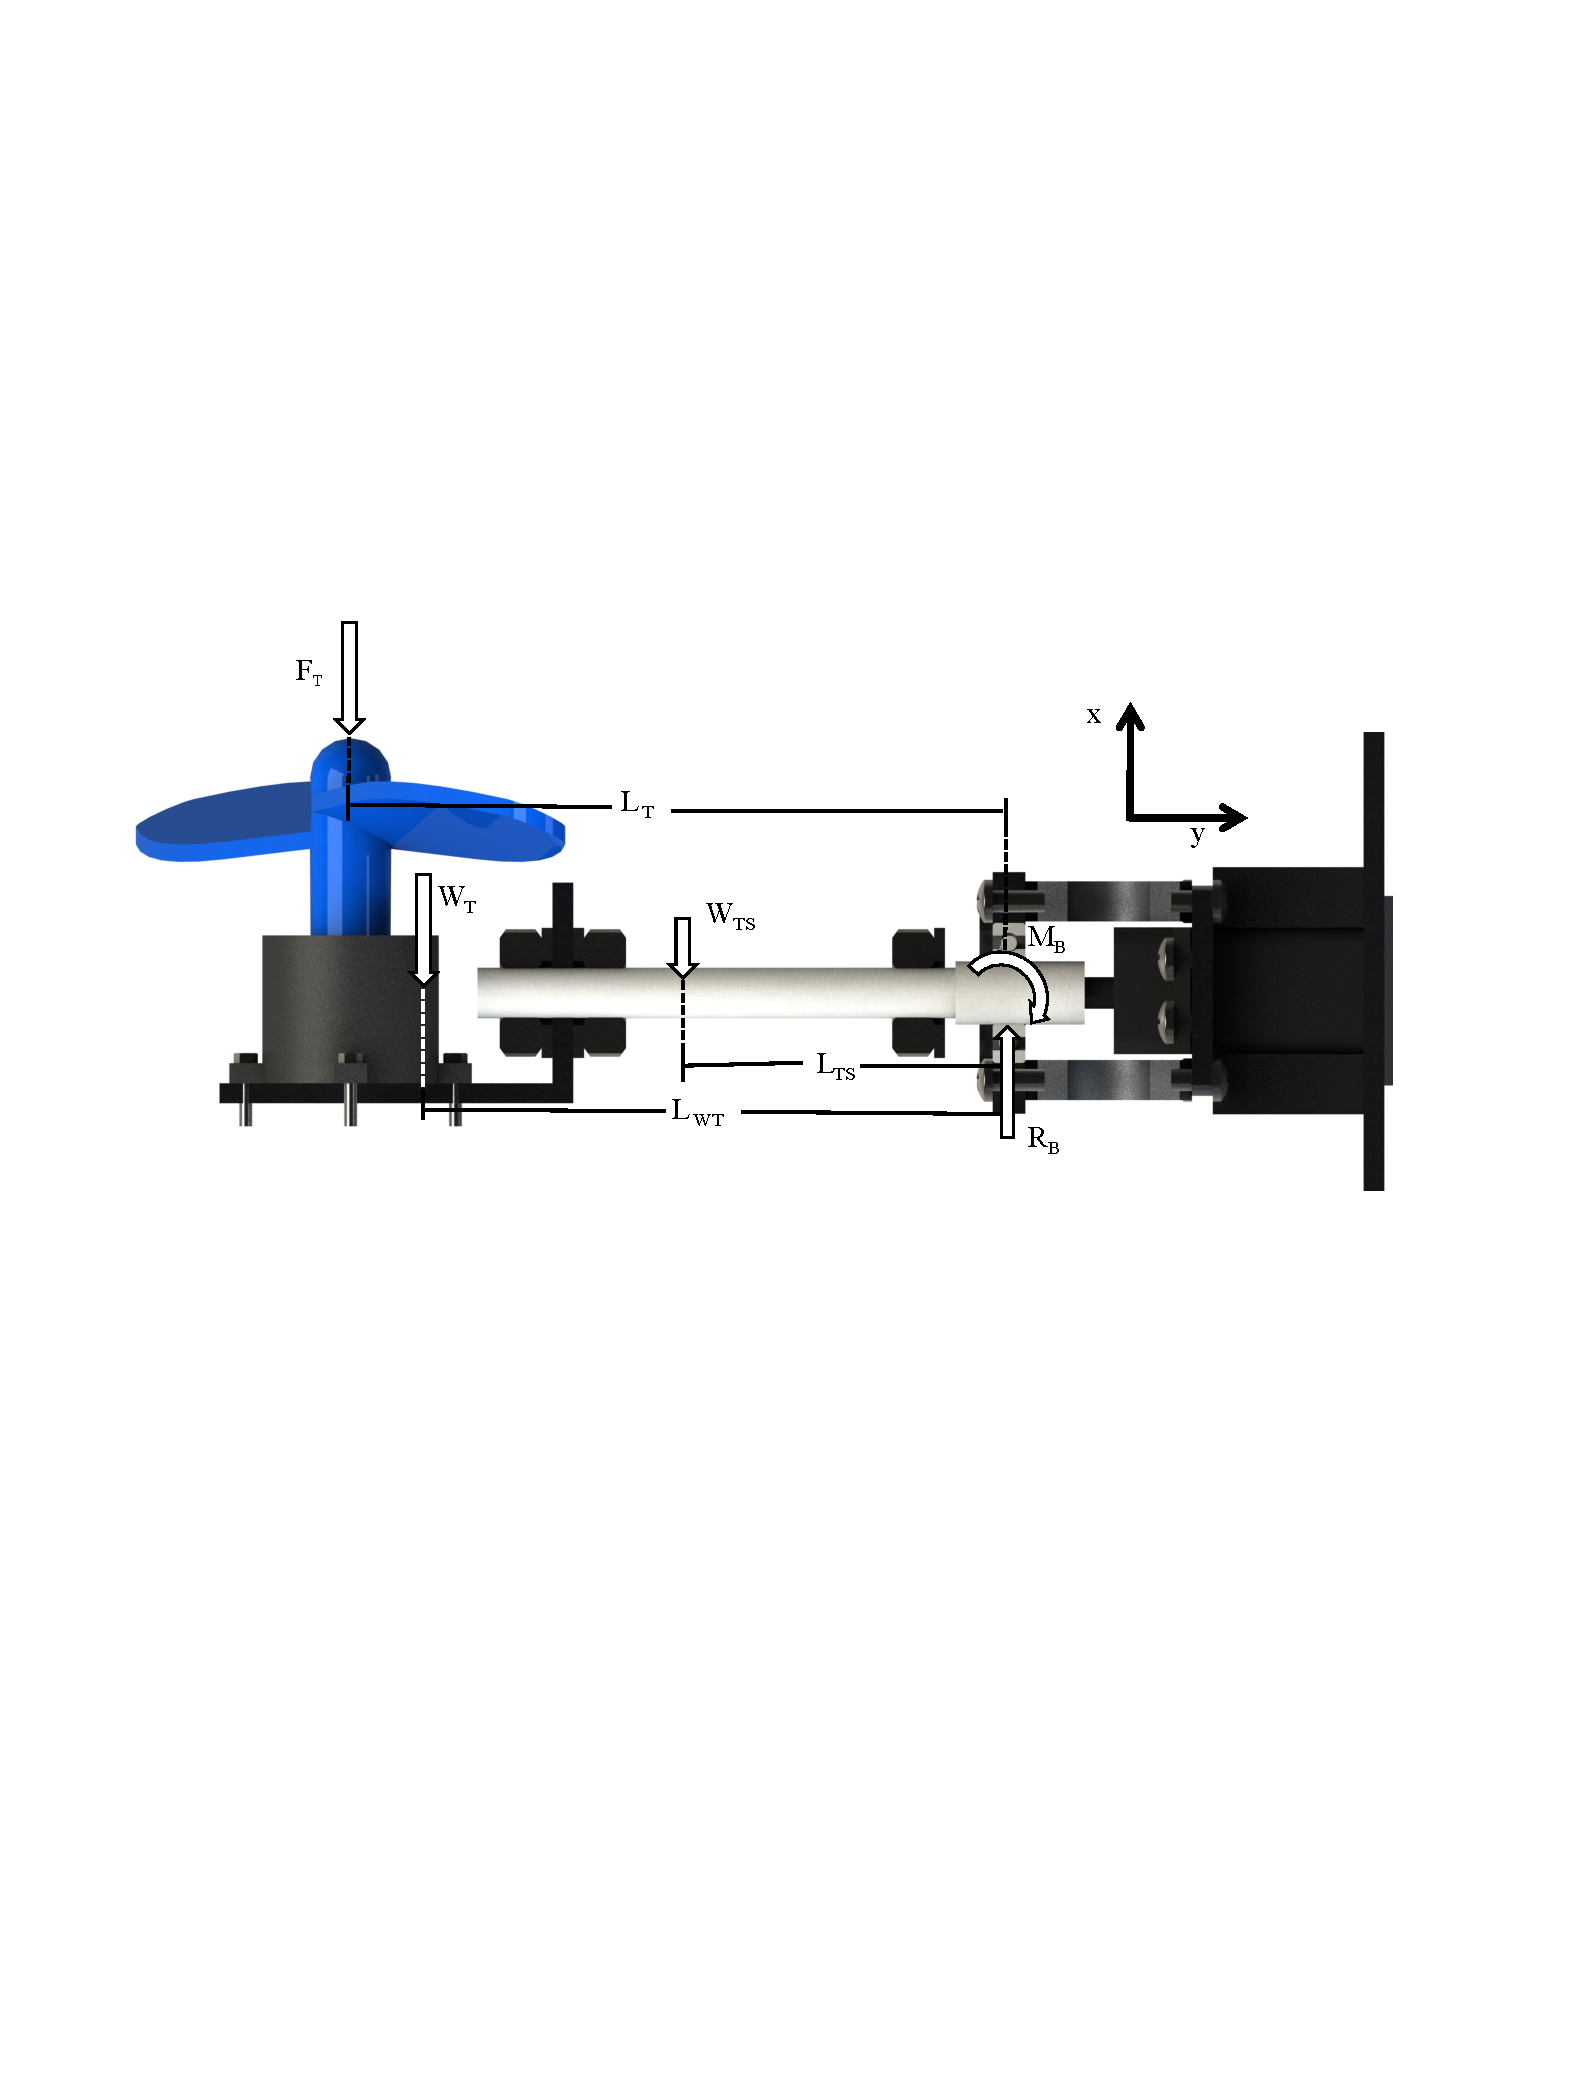
\includegraphics[width=.9\linewidth]{img/analysis/thruster/thrusterShaft.pdf}
	\caption{Free Body of the Thruster Shaft}
	\label{fig:thrusterShaftFBD}
\end{figure}

The free body diagram in Figure \ref{fig:thrusterShaftFBD} is used to get the summation of forces at the bearing. The forces on the figure are the thrust force ($F_T$), weight of thruster components ($W_T$), weight of shaft ($W_{TS}$), and the reaciton forces ($R_B$ and $M_B$). As mentioned the forceSolver REF?? does this analysis, however calculating by hand will need the summation of forces:

\begin{equation}
\label{eqn:thrustShaftFx} 
\upplus \Sigma F_x  = 0 = R_B - F_T - W_T - W_{TS}
\end{equation}
\begin{equation}
\label{eqn:thrustShaftMB} 
\curveplus \Sigma M_B = 0 = -M_B + F_T(L_T) - W_T(L_{WT}) - W_{TS}(L_{TS})
\end{equation}

Because in this scenario both the thrust and the weight are acting in the same direction all forces are acting in the x-direction. So the greatest stress will be the one generated by the moment in $z$ ($M_B$). Stress is calculated using the equation \ref{eqn:thrustShaftStress} shown below, assuming that the maximum stress will occur when the shaft is in tension at the upper outer edge. Where $c$ is the radius to the maximum pitch and $I_z$ is the moment of inertia in z of a hollow cylinder (Equation \ref{eqn:hollowInertia}).

\begin{equation}
\label{eqn:thrustShaftStress} 
\sigma _{Shaft}  = \dfrac{M_{B}c}{I_z} 
\end{equation}

\begin{equation}
\label{eqn:hollowInertia} 
I _{z}  = \dfrac{\pi}{4} (r_{minor}^4 - r_{bore}^4)
\end{equation}

Since this is only simple bending the analysis does not have to use Cauchy to solve the stresses. However Brittle Mohr-Coulomb Theory \cite[227]{shigley} can still be used with the only stress being plugged in. In equation $\sigma_{t}$ is the ultimate tensile strength of Nylon 6 \cite{Nylon6}.

\begin{equation}
\eta = \dfrac{\sigma_{T}}{\sigma _a} \Rightarrow 3 \geq \dfrac{\sigma_{T}}{\sigma _a}
\end{equation}

<<<<<<< HEAD
Due to the medium failure likelihood a safety factor $\eta$ of 3 is used. If for the shaft diameter used does not meet this requirement, the code selects the next highest standard threaded shaft diameter and runs through the analysis using those numbers. This repeats until the safety factor is met. 

\subsubsection*{Sample Calculations}
$M_z$ is calculated using the MATLAB Force Solver program.
$$\sigma _{Shaft}  = \dfrac{M_{z}c}{I} = \dfrac{(1.2535N\cdot{}m)(0.0051m)}{(3.4817\cdot{}10^{-10}mm^4)}=18.28MPa$$
$$I _{z}  = \dfrac{\pi}{4} (r_{minor}^4 - r_{bore}^4) = \dfrac{\pi}{4} ((0.0051mm)^4 - (0.0038)^4) = 3.4817\cdot{}10^{-10}mm^4$$
$$\eta = \dfrac{S_{ut}}{\sigma _a} \Rightarrow 3 \geq \dfrac{S_{ut}}{\sigma _a}$$
$$\eta = \dfrac{69MPa}{18.28MPa}=3.7756$$
After 3 iterations, a safety factor of 3.8 is calculated which has gone above the design threshold.
=======
Due to the medium failure likelihood, a safety factor $\eta$ of 3 is used. If for the shaft diameter used does not meet this requirement, the code selects the next highest standard threaded shaft diameter and runs through the analysis using those numbers. This repeats until the safety factor is met. 
>>>>>>> 6d7ea59e7b65f6b9a259f8e5d0ea953ddb63870b
\end{document}